% vim: set spell spelllang=en tw=100 et sw=4 sts=4 :

\documentclass{llncs}

% \usepackage{showframe}

\usepackage{microtype}
\usepackage{complexity}                % \P, \NP etc
\usepackage{tikz}                      % For pretty pictures
\usepackage{amsmath}                   % \operatorname
\usepackage{hyperref}                  % clicky links
\usepackage{cleveref}                  % no need to type Figure etc
\usepackage{gnuplot-lua-tikz}          % graphs
\usepackage[ruled,vlined]{algorithm2e} % algorithms (after cleverref!)
\usepackage{placeins}                  % \FloatBarrier
\usepackage{cite}
\usepackage[bottom]{footmisc}

\usetikzlibrary{arrows, shadows, calc, positioning, decorations, decorations.pathreplacing, patterns}

% lncs style
\crefname{algocf}{Algorithm}{Algorithms}
\Crefname{algocf}{Algorithm}{Algorithms}
\crefname{figure}{Fig.}{Figs.}
\Crefname{figure}{Fig.}{Figs.}
\crefname{table}{Table}{Tables}
\Crefname{table}{Table}{Tables}
\crefname{proposition}{Proposition}{Propositions}
\Crefname{proposition}{Proposition}{Propositions}

\newcommand{\lineref}[1]{line~\ref{#1}}
\newcommand{\twolinesref}[2]{lines~\ref{#1} and~\ref{#2}}

\newcommand*\samethanks[1][\value{footnote}]{\footnotemark[#1]}

\title{Clique and Constraint Models for Maximum Common (Connected) Subgraph Problems}

\author{Ciaran McCreesh\thanks{This work was supported by the Engineering and Physical Sciences
    Research Council [grant number EP/K503058/1]}\inst{1} \and Samba Ndojh Ndiaye\thanks{This work
was supported by the ANR project SoLStiCe (ANR-13-BS02-0002-01)}\inst{2} \and Patrick
Prosser\inst{1} \and Christine Solnon\samethanks[2] \inst{3}}
\institute{University of Glasgow, Glasgow, Scotland \and
Universit\'e Lyon 1, LIRIS, UMR5205, F-69621, France  \and INSA-Lyon, LIRIS, UMR5205, F-69621, France}

\begin{document}

\maketitle

\begin{abstract}
    The maximum common subgraph problem is to find the largest subgraph common to two given graphs.
    This problem can be solved either by constraint-based search, or by reduction to the maximum
    clique problem. We evaluate these two approaches using modern algorithms. We also propose a
    restricted branching approach for the connected version of the problem, show how to implement
    this in constraint-based and clique-inspired algorithms, and compare it to conventional
    propagation.
\end{abstract}

\section{Introduction}

\begin{figure}[b] % first page if possible
    \centering
    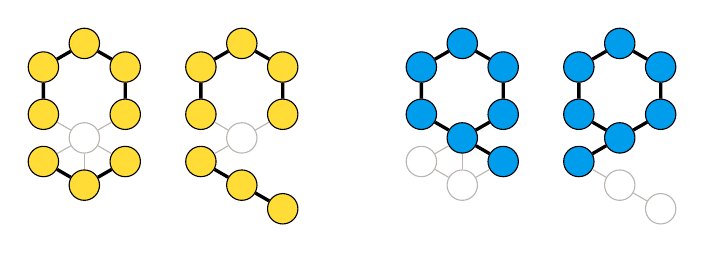
\begin{tikzpicture}[scale=0.4]%{{{
        \definecolor{uofgcobalt}{rgb}{0, 0.615686, 0.92549}
        \definecolor{uofgsunshine}{rgb}{1.0, 0.862745, 0.211765}
        \definecolor{uofgsandstone}{rgb}{0.321569, 0.278431, 0.231373}
        \begin{scope}
            \node[draw, circle, fill=uofgsunshine, inner sep=1pt, font=\normalsize] (M1) at (90:1.5) {\phantom{0}};
            \node[draw, circle, fill=uofgsunshine, inner sep=1pt, font=\normalsize] (M2) at (150:1.5) {\phantom{0}};
            \node[draw, circle, fill=uofgsunshine, inner sep=1pt, font=\normalsize] (M3) at (30:1.5) {\phantom{0}};
            \node[draw, circle, fill=uofgsunshine, inner sep=1pt, font=\normalsize] (M4) at (210:1.5) {\phantom{0}};
            \node[draw, circle, fill=uofgsunshine, inner sep=1pt, font=\normalsize] (M5) at (330:1.5) {\phantom{0}};
            \node[draw, circle, draw=uofgsandstone!40, fill=white, inner sep=1pt, font=\normalsize] (M6) at (270:1.5) {\phantom{0}};
            \node[draw, circle, fill=uofgsunshine, inner sep=1pt, font=\normalsize] (M7) at ($(210:1.5) + (M6)$) {\phantom{0}};
            \node[draw, circle, fill=uofgsunshine, inner sep=1pt, font=\normalsize] (M8) at ($(330:1.5) + (M6)$) {\phantom{0}};
            \node[draw, circle, fill=uofgsunshine, inner sep=1pt, font=\normalsize] (M9) at ($(270:1.5) + (M6)$) {\phantom{0}};

            \draw [very thick] (M1) -- (M2);
            \draw [very thick] (M2) -- (M4);
            \draw [very thick] (M3) -- (M5);
            \draw [color=uofgsandstone!40] (M4) -- (M6);
            \draw [color=uofgsandstone!40] (M5) -- (M6);
            \draw [very thick] (M3) -- (M1);
            \draw [color=uofgsandstone!40] (M6) -- (M7);
            \draw [color=uofgsandstone!40] (M6) -- (M8);
            \draw [color=uofgsandstone!40] (M6) -- (M9);
            \draw [very thick] (M7) -- (M9);
            \draw [very thick] (M8) -- (M9);
        \end{scope}

        \begin{scope}[xshift=5cm]
            \node[draw, circle, fill=uofgsunshine, inner sep=1pt, font=\normalsize] (M1) at (90:1.5) {\phantom{0}};
            \node[draw, circle, fill=uofgsunshine, inner sep=1pt, font=\normalsize] (M2) at (150:1.5) {\phantom{0}};
            \node[draw, circle, fill=uofgsunshine, inner sep=1pt, font=\normalsize] (M3) at (30:1.5) {\phantom{0}};
            \node[draw, circle, fill=uofgsunshine, inner sep=1pt, font=\normalsize] (M4) at (210:1.5) {\phantom{0}};
            \node[draw, circle, fill=uofgsunshine, inner sep=1pt, font=\normalsize] (M5) at (330:1.5) {\phantom{0}};
            \node[draw, circle, draw=uofgsandstone!40, fill=white, inner sep=1pt, font=\normalsize] (M6) at (270:1.5) {\phantom{0}};
            \node[draw, circle, fill=uofgsunshine, inner sep=1pt, font=\normalsize] (M7) at ($(210:1.5) + (M6)$) {\phantom{0}};
            \node[draw, circle, fill=uofgsunshine, inner sep=1pt, font=\normalsize] (M8) at ($(270:1.5) + (M6)$) {\phantom{0}};
            \node[draw, circle, fill=uofgsunshine, inner sep=1pt, font=\normalsize] (M9) at ($(330:1.5) + (M8)$) {\phantom{0}};

            \draw [very thick] (M1) -- (M2);
            \draw [very thick] (M2) -- (M4);
            \draw [very thick] (M3) -- (M5);
            \draw [color=uofgsandstone!40] (M4) -- (M6);
            \draw [color=uofgsandstone!40] (M5) -- (M6);
            \draw [very thick] (M3) -- (M1);
            \draw [color=uofgsandstone!40] (M6) -- (M7);
            \draw [very thick] (M7) -- (M8);
            \draw [very thick] (M8) -- (M9);
        \end{scope}

        \begin{scope}[xshift=12cm]
            \node[draw, circle, fill=uofgcobalt, inner sep=1pt, font=\normalsize] (M1) at (90:1.5) {\phantom{0}};
            \node[draw, circle, fill=uofgcobalt, inner sep=1pt, font=\normalsize] (M2) at (150:1.5) {\phantom{0}};
            \node[draw, circle, fill=uofgcobalt, inner sep=1pt, font=\normalsize] (M3) at (30:1.5) {\phantom{0}};
            \node[draw, circle, fill=uofgcobalt, inner sep=1pt, font=\normalsize] (M4) at (210:1.5) {\phantom{0}};
            \node[draw, circle, fill=uofgcobalt, inner sep=1pt, font=\normalsize] (M5) at (330:1.5) {\phantom{0}};
            \node[draw, circle, fill=uofgcobalt, inner sep=1pt, font=\normalsize] (M6) at (270:1.5) {\phantom{0}};
            \node[draw, circle, draw=uofgsandstone!40, fill=white, inner sep=1pt, font=\normalsize] (M7) at ($(210:1.5) + (M6)$) {\phantom{0}};
            \node[draw, circle, fill=uofgcobalt, inner sep=1pt, font=\normalsize] (M8) at ($(330:1.5) + (M6)$) {\phantom{0}};
            \node[draw, circle, draw=uofgsandstone!40, fill=white, inner sep=1pt, font=\normalsize] (M9) at ($(270:1.5) + (M6)$) {\phantom{0}};

            \draw [very thick] (M1) -- (M2);
            \draw [very thick] (M2) -- (M4);
            \draw [very thick] (M3) -- (M5);
            \draw [very thick] (M4) -- (M6);
            \draw [very thick] (M5) -- (M6);
            \draw [very thick] (M3) -- (M1);
            \draw [color=uofgsandstone!40] (M6) -- (M7);
            \draw [very thick] (M6) -- (M8);
            \draw [color=uofgsandstone!40] (M6) -- (M9);
            \draw [color=uofgsandstone!40] (M7) -- (M9);
            \draw [color=uofgsandstone!40] (M8) -- (M9);
        \end{scope}

        \begin{scope}[xshift=17cm]
            \node[draw, circle, fill=uofgcobalt, inner sep=1pt, font=\normalsize] (M1) at (90:1.5) {\phantom{0}};
            \node[draw, circle, fill=uofgcobalt, inner sep=1pt, font=\normalsize] (M2) at (150:1.5) {\phantom{0}};
            \node[draw, circle, fill=uofgcobalt, inner sep=1pt, font=\normalsize] (M3) at (30:1.5) {\phantom{0}};
            \node[draw, circle, fill=uofgcobalt, inner sep=1pt, font=\normalsize] (M4) at (210:1.5) {\phantom{0}};
            \node[draw, circle, fill=uofgcobalt, inner sep=1pt, font=\normalsize] (M5) at (330:1.5) {\phantom{0}};
            \node[draw, circle, fill=uofgcobalt, inner sep=1pt, font=\normalsize] (M6) at (270:1.5) {\phantom{0}};
            \node[draw, circle, fill=uofgcobalt, inner sep=1pt, font=\normalsize] (M7) at ($(210:1.5) + (M6)$) {\phantom{0}};
            \node[draw, circle, draw=uofgsandstone!40, fill=white, inner sep=1pt, font=\normalsize] (M8) at ($(270:1.5) + (M6)$) {\phantom{0}};
            \node[draw, circle, draw=uofgsandstone!40, fill=white, inner sep=1pt, font=\normalsize] (M9) at ($(330:1.5) + (M8)$) {\phantom{0}};

            \draw [very thick] (M1) -- (M2);
            \draw [very thick] (M2) -- (M4);
            \draw [very thick] (M3) -- (M5);
            \draw [very thick] (M4) -- (M6);
            \draw [very thick] (M5) -- (M6);
            \draw [very thick] (M3) -- (M1);
            \draw [very thick] (M6) -- (M7);
            \draw [draw=uofgsandstone!40] (M7) -- (M8);
            \draw [draw=uofgsandstone!40] (M8) -- (M9);
        \end{scope}
\end{tikzpicture}
\caption{A maximum common induced subgraph of the first two graphs has eight vertices. There are
four symmetric solutions, all involving the shaded vertices. However, if we require the common
subgraph to be connected, only seven vertices may be selected---one way to do this is shown in the
third and fourth graphs.}\label{figure:mcsexample}
\end{figure}

A common subgraph of two graphs is a graph which is subgraph-isomorphic to both graphs---we
illustrate this concept in \cref{figure:mcsexample}, and define this formally below. Finding a
maximum common subgraph gives a measure of the similarity between two graphs, and allows for the
edit distance to be computed ?? cite. Maximum common subgraph problems have applications in
chemistry, computer vision, ?? cite.

One approach to this problem is via constraint programming (CP) models
\cite{DBLP:conf/cp/NdiayeS11}. These models are based upon constructing an injective mapping from
the vertices of one graph (typically the smaller) to the other, in a similar manner to subgraph
isomorphism algorithms ?? cite. However, to allow for a partial mapping, a special null value is
added to each domain (and the injectivity condition does not apply to null values). The problem then
becomes an optimisation problem, where we seek to minimise the number of null values. ?? find a way
to work weak all diff in here. Unfortunately, this null value invalidates many of the invariants
used for subgraph isomorphism---we may no longer reason using the degree of vertices, or the
distances between them, for example, and so the problem can be much more challenging in practice.

Another popular approach is to reduce the problem to finding a maximum clique (or sometimes,
equivalently, an independent set or a vertex cover) in an association graph (which we describe
below). This seems to be less effective in practice, but previous experimental evaluations have used
weak clique algorithms, or even clique enumeration algorithms. Maximum clique algorithms are an
active research area
\cite{DBLP:conf/dmtcs/TomitaS03,DBLP:journals/jgo/TomitaK07,DBLP:conf/walcom/TomitaSHTW10,DBLP:journals/cor/SegundoRJ11,DBLP:journals/algorithms/Prosser12,DBLP:journals/ol/SegundoMRH13,DBLP:conf/ictai/LiFX13,DBLP:journals/cor/SegundoT14,DBLP:conf/lion/SegundoLB14,DBLP:conf/cp/McCreeshP14,DBLP:journals/jco/BatsynGMP14,DBLP:journals/cor/SegundoNB15,DBLP:conf/lion/NikolaevBS15,DBLP:conf/lion/LiJX15,DBLP:journals/jcc/KoncDTRJ12,DBLP:journals/algorithms/McCreeshP13,DBLP:journals/topc/McCreeshP15,DBLP:journals/cor/SegundoLP16},
and so the first half of this paper re-evaluates this approach using a modern algorithm.

(Other approaches have been tried, including MIP ?? cite, SAT.)

A particularly challenging variant of the maximum common subgraph problem requires the selected
subgraph to be connected \cite{DBLP:journals/tcs/Koch01,DBLP:conf/mco/VismaraV08}. The second half
of the paper looks at this variant. In principle, for a CP approach, we may simply add a ``forms a
connected graph'' global constraint to the model. However, we will show that better results may be
obtained via a special branching rule. We then explain how to adapt this branching rule to run
inside a clique-like algorithm, to solve the problem via an association graph.

\subsection{Definitions and Notation}

A \emph{graph} $G = (V, E)$ consists of a set of vertices $V$ and a set of edges $E \subseteq V
\times V$. In this paper our graphs may be directed, may have loops, and there is a label associated
with each vertex and with each edge. For convenience, we treat undirected graphs as being directed
graphs with symmetric adjacencies, and for unlabelled graphs we treat each vertex as having the same
label, and each edge as having the same label. We write $\operatorname{V}(G)$ for $V$, and
$\operatorname{N}(G, v)$ for the \emph{undirected neighbourhood} of a vertex $v$ (that is, the set
of vertices $w$ such that either $(v, w)$ or $(w, v)$ is an edge).

Given two graphs $G_1$ and $G_2$, we say two pairs of vertices $(v_1, w_1) \in \operatorname{V}(G_1)
\times \operatorname{V}(G_1)$ and $(v_2, w_2) \in \operatorname{V}(G_2) \times
\operatorname{V}(G_2)$ are \emph{compatible} if both $v_1$ and $w_1$ and $v_2$ and $w_2$ are either
non-adjacent or adjacent with the same label, and if the same holds for $(w_1, v_1)$ and $(w_2,
v_2)$.  We say two vertices $v \in \operatorname{V}(G_1)$ and $w \in \operatorname{V}(G_2)$ are
\emph{compatible} if they share the same label, and $(v, v)$ is compatible with $(w, w)$.

\subsection{Datasets}

\cite{DBLP:journals/prl/SantoFSV03,DBLP:journals/jgaa/ConteFV07}

\section{Re-Evaluating the Clique Model}

Previous experimental work has used a maximal clique enumeration algorithm, even for the
maximisation problem. ?? check this! I recall someone using a bad max clique algorithm too.
\cite{DBLP:conf/sspr/BunkeFGSV02,DBLP:journals/jgaa/ConteFV07}

We instead use a maximum clique algorithm. There has been a lot of recent
research on this
.

Also sparse stuff, but association graphs aren't sparse enough.

Say which clique algorithm we're using.

\subsection{Reduction to Maximum Clique in an Association Graph}

Explain association graph. ?? cite history, connections to microstructure

Discuss how edge labels, vertex labels, directed edges, etc, are handled. Note that we can generally
only handle very local side constraints, or injectivity (which is decomposable).

\subsection{Experimental Evaluation}

\cref{figure:unconnected-33}

\cref{figure:unconnected-plain}

\begin{figure}[p]
    \centering
    \input{gen-graph-unconnected-33}
    \caption{Clique versus CP, 33\% labelled. On the top, the cumulative
    number of instances solved by each approach, in under a certain time. On the bottom, the best
    clique approach compared to the best CP approach: the colour at a point indicates the number of
    instances with these runtimes.} \label{figure:unconnected-33}
\end{figure}

\begin{figure}[p]
    \centering
    \input{gen-graph-unconnected-plain}
    \caption{Clique versus CP, undirected, unlabelled. On the top, the cumulative
    number of instances solved by each approach, in under a certain time. On the bottom, the best
    clique approach compared to the best CP approach: the colour at a point indicates the number of
    instances with these runtimes.} \label{figure:unconnected-plain}
\end{figure}

\subsection{Parallel Search}

\cite{DBLP:journals/jcc/KoncDTRJ12,DBLP:journals/algorithms/McCreeshP13,DBLP:journals/topc/McCreeshP15,DBLP:journals/cor/SegundoLP16}

?? Stuff on EHPs, how work stealing matters here too \cite{DBLP:journals/jco/BatsynGMP14}

\section{Maximum Common Connected Subgraph}

Connectedness is not hereditary, but can be built up one vertex at a time. Alternatively,
connectedness is a constraint.

\subsection{Connectedness as a Constraint}

Connectedness \cite{Brown:2005}

Reachability \cite{DBLP:conf/cp/DoomsDD05,DBLP:conf/cp/QuesadaRD05}

\subsection{Connectedness via Restricted Branching}

The key idea is that whenever we branch (except for the first choice we make), we select only from
variables which correspond to vertices which are adjacent to at least one other variable which has
been instantiated to a non-null value. If no such variables remain, the subgraph we are building
cannot grow any further, and all remaining variables must be instantiated to null.

?? We only need to work off whichever input gives us the variables. But the CP approach seems to
look at both?

?? Patrick reckons this reminds him of Prim's algorithm for minimum spanning trees.

?? We need a picture here.

\subsection{Connectedness in an Association Graph Algorithm}

\begin{algorithm}[p] \DontPrintSemicolon
\nl $\FuncSty{associationMCCIS}$ :: (Graph $G_1$, Graph $G_2$) $\rightarrow$ Map \;
\nl \Begin{
    \nl $\KwSty{global} ~ \mathit{incumbent} \gets \emptyset$ \label{incumbent} \;
    \nl $G \gets \FuncSty{associationGraph}(G_1, G_2)$ \label{buildassoc} \;
    \nl $\FuncSty{search}(G, \emptyset, \emptyset, \operatorname{V}(G))$ \label{firstsearch} \;
    \nl $\KwSty{return} ~ \mathit{incumbent}$ \;
}
\vspace{1ex}
\nl $\FuncSty{search}$ :: (Graph $G$, Set $\mathit{solution}$, Set $\mathit{branchable}$, Set $\mathit{remaining}$) \;
\nl \Begin{
    \nl $\mathit{colourClasses} \gets \FuncSty{concatenate}($ \label{makecolours} \;
    $\hspace*{2em}\FuncSty{colour}(G, \mathit{remaining} \setminus \mathit{branchable}),$ \;
    $\hspace*{2em}\FuncSty{colour}(G, \mathit{remaining} \cap \mathit{branchable}))$ \;
    \nl \While{$\FuncSty{length}(\mathit{colourClasses}) > 0$\label{outerloop}}{
        \nl \ForEach{$v \in \FuncSty{last}(\mathit{colourClasses}) \textnormal{~in reverse order}$\label{innerloop}}{
            \nl \lIf{$|\mathit{solution}| + \FuncSty{length}(\mathit{colourClasses}) \leq
            |\mathit{incumbent}|$}{\KwSty{return}\label{bound}}
            \nl \lIf{$v \notin \mathit{branchable} ~ \KwSty{and} ~ \mathit{solution} \ne
            \emptyset$}{\KwSty{return} \label{acceptbranchable}}
            \nl $\mathit{solution}' \gets \mathit{solution} \cup \{ v \} \label{addv} \label{addvtosolution} $\;
            \nl \lIf{$|\mathit{solution}'| > |\mathit{incumbent}|$}{$\mathit{incumbent} \gets
            \mathit{solution}'$ \label{newincumbent}}
            \nl $\mathit{branchable}' \gets \mathit{branchable} \cup \FuncSty{connected}(G, v)$ \label{addtobranchable} \;
            \nl $\mathit{remaining}' \gets \mathit{remaining} \cap \operatorname{N}(G, v)$ \label{filterremaining} \;
            \nl \lIf{$\mathit{remaining}' \neq \emptyset$}{$\FuncSty{search}(G, \mathit{solution}',
            \mathit{branchable}', \mathit{remaining}')$\label{recursesearch}}
         }
         \nl $\FuncSty{removeLast}(\mathit{colourClasses})$ \;
     }
}
\vspace{1ex}
\nl $\FuncSty{colour}$ :: (Graph $G$, Set $\mathit{uncoloured}$) $\rightarrow$ List of List of Vertex \;
\nl \Begin{
    \nl $\mathit{result} \gets []$ \;
    \nl \While{$\mathit{uncoloured} \ne \emptyset$\label{whileuncoloured}}{
        \nl $\mathit{colourClass} \gets []$ \label{newcolourclass} \;
        \nl $\mathit{colourable} \gets \mathit{uncoloured}$ \;
        \nl \While{$\mathit{colourable} \ne \emptyset$}{
            \nl $v \gets \textnormal{the first vertex from}~\mathit{uncoloured}~\textnormal{by
            static degree order from}~G$ \label{selectvtocolour} \;
            \nl $\FuncSty{append}(\mathit{colourClass}, v)$ \label{addtocolourclass} \;
            \nl $uncoloured \gets uncoloured \setminus \{ v \}$ \;
            \nl $\mathit{colourable} \gets \mathit{colourable} \setminus \operatorname{N}(G, v)$ \;
        }
        \nl $\FuncSty{append}(\mathit{result}, \mathit{colourClass})$ \;
    }
    \nl $\KwSty{return} ~ \mathit{result}$ \;
}
\vspace{1ex}
\nl $\FuncSty{connected}$ :: (Graph $G$, Vertex $v$) $\rightarrow$ Set \;
\nl \Begin{
    \nl $\KwSty{return} ~ \{ w \in G : \FuncSty{first}(w) \in \operatorname{N}(G, \FuncSty{first}(v)) \}$ \;
}
\vspace{1ex}
\nl $\FuncSty{associationGraph}$ :: (Graph $G_1$, Graph $G_2$) $\rightarrow$ Graph \;
\nl \Begin{
    \nl $V \gets \{ (v_1, v_2) \in G_1 \times G_2 : \FuncSty{compatible}(v_1, v_2) \}$ \;
    \nl $E \gets \{ ((v_1, v_2), (w_1, w_2)) \in V \times V : \FuncSty{compatible}((v_1, w_1), (v_2,
    w_2)) \}$ \;
    \nl $\KwSty{return} ~ (V, E)$ \;
}
\caption{An algorithm for MCCIS via an association graph.}
\label{algorithm:mccis}
\end{algorithm}

It is not possible to determine connectedness from a raw association graph. However, we can take a
maximum clique algorithm and mimic the branching strategy if we have access to the underlying graphs
and can determine the ``meaning'' of the association graph vertices.

Most modern maximum clique algorithms for dense graphs use some variation of greedy graph colouring
as a bound---the underlying observation is that each vertex in a clique must be given a different
colour in a colouring, so if we can colour a subset of vertices using $k$ colours then a maximum
clique in this subset has at most $k$ vertices. However, the colouring is also used as a branching
heuristic: vertices are selected in reverse from their colour classes in turn, starting with the
last colour class created. Because of this coupling of branching and the bound (which is important
in practice because it mimics a ``smallest domain first'' branching heuristic if colour classes are
viewed as variables \cite{DBLP:conf/cp/McCreeshP14}), if we were to select only a subset of vertices for
branching at each stage inside a clique algorithm, we would lose completeness. Thus we must adapt
the bound to take into account restricted branching.

In \cref{algorithm:mccis} we present a clique-inspired algorithm which finds an MCCIS via an
association graph. If the additional
branching restrictions are removed, the core of the algorithm is what Prosser
\cite{DBLP:journals/algorithms/Prosser12} calls the ``MCSa1'' variant of a series of algorithms due
to Tomita \textit{et al.}\
\cite{DBLP:conf/dmtcs/TomitaS03,DBLP:journals/jgo/TomitaK07,DBLP:conf/walcom/TomitaSHTW10}, using a
bitset encoding approach due to San Segundo \textit{et al.}\
\cite{DBLP:journals/cor/SegundoRJ11,DBLP:journals/ol/SegundoMRH13} (and we refer the reader to these
papers for implementation details on how to use bitsets and other data structures to implement the
colouring stage with very low constant factors).

We begin by building the association graph (\lineref{buildassoc}). The main part of the algorithm
then works by building up candidate cliques in the $\mathit{solution}$ variable, by recursive calls
to the $\mathit{search}$ procedure---starting from the empty set (\lineref{firstsearch}), each
recursive subcall adds one vertex to $\mathit{solution}$ (\lineref{addv}) in such a way that
$\mathit{solution}$ is always a clique which corresponds to a connected common subgraph. The
$\mathit{remaining}$ set contains the set of vertices which are adjacent to every vertex in
$\mathit{solution}$, and which have not yet been accepted or rejected (and so initially it contains
every vertex). The main loops in the $\FuncSty{search}$ procedure
(\twolinesref{outerloop}{innerloop}) have the effect of iterating over each vertex in this set in a
particular order---each vertex $v$ is selected in turn, and then a recursive call is made to
consider the effects of including $v$ in $\mathit{solution}$ (\lineref{recursesearch}), followed by
the next iteration where $v$ is instead rejected. When $v$ is accepted, we add it to the new
$\mathit{solution'}$ (\lineref{addvtosolution}), and create a new $\mathit{remaining'}$ containing
only the vertices in $\mathit{remaining}$ which are adjacent to $v$ (\lineref{filterremaining}).

The $\mathit{branchable}$ set contains the set of association graph vertices which correspond to
vertices adjacent to an already-accepted vertex in the first input graph---in CP terms, it is the
set of assignments which could be made next which preserve connectedness. (Using only one of the two
input graphs is sufficient for correctness, and has the advantage that the $\FuncSty{connected}$
function may be implemented as a simple lookup into a precomputed array which maps each vertex in
the first input graph to a bitset.) At the top of search, this set is empty, and is not used (our
first vertex selection is special, and does not care about connectedness). At subsequent depths, we
may only accept vertices which are in this set, and if no such vertices remain then we return
immediately (\lineref{acceptbranchable}). When recursing, we extend $\mathit{branchable}$ with the
new vertices permitted by our acceptance of the branching $v$ (\lineref{addtobranchable}). Note that
we are assuming that inside the main loops, we encounter every vertex in $\mathit{remaining} \cap
\mathit{connected}$ before any vertex in $\mathit{remaining} \setminus \mathit{connected}$.

As we proceed, we keep track of the best solution we have found so far---this is stored in the
$\mathit{incumbent}$ variable (\twolinesref{incumbent}{newincumbent}). We use the incumbent,
together with a colour bound, to prune portions of the search space which cannot contain a better
solution. The colour bound operates as follows: at each entry to the $\FuncSty{search}$ procedure,
we produce a greedy colouring of the vertices in $\mathit{remaining}$ (\lineref{makecolours}). This
greedy colouring gives us a list of colour classes, each of which is a list of pairwise non-adjacent
vertices. The two loops (\twolinesref{outerloop}{innerloop}) then iterate over each colour class,
from last to first, and then over each vertex in that colour class, again from last to first.
(Rather than actually using a list of lists and removing items, this process should be implemented
using a pair of immutable flat arrays. This technique is described elsewhere
\cite{DBLP:conf/cp/McCreeshP14}, so we do not discuss it here.) Finally, if at any point the number
of remaining colour classes plus the number of vertices currently present in $\mathit{solution}$ is
not strictly greater than the size of the incumbent, then we may backtrack immediately
(\lineref{bound}).

Finally, we describe the colouring process. In conventional clique algorithms, a simple greedy
sequential colouring is used (possibly with the help of previous colourings to reduce the
computational cost \cite{DBLP:conf/lion/NikolaevBS15}, and possibly with shortcuts taken for certain
vertices \cite{DBLP:journals/cor/SegundoT14}, and possibly followed by a repair step to
improve the colouring \cite{DBLP:conf/walcom/TomitaSHTW10}, or stronger bounding rules based upon
MaxSAT inference \cite{DBLP:conf/ictai/LiFX13,DBLP:conf/lion/LiJX15,DBLP:journals/cor/SegundoNB15}).
Such colourings will not give us the required property that vertices in $\mathit{remaining} \cap
\mathit{connected}$ come last (so they are selected first by the reverse branching order). Thus we
produce two greedy sequential colourings, first considering the non-branching vertices in
$\mathit{remaining} \setminus \mathit{connected}$, followed by the branching vertices, and
concatenate them (\lineref{makecolours}). This produces a valid colouring, since we do not merge any
colour classes between the two stages, although it may use more colours than a single colouring
would.

Our $\FuncSty{colour}$ procedure is the same as the bit-parallel algorithm introduced by San Segundo
\textit{et al.}\ \cite{DBLP:journals/cor/SegundoRJ11}. While we have remaining vertices to colour
(\lineref{whileuncoloured}), we start a new colour class (\lineref{newcolourclass}), and then
repeatedly pick a legal vertex to add to that colour class (\lineref{addtocolourclass}).  The
selection of the next vertex to colour (\lineref{selectvtocolour}) may be performed efficiently in
hardware if the association graph is permuted to be in degree order at the top of search. (Other
initial vertex orderings have been considered on general clique problems
\cite{DBLP:journals/algorithms/Prosser12,DBLP:conf/lion/SegundoLB14}; it is possible that special
properties of the association graph could be exploited in this step.)

\subsection{Experimental Evaluation}

\paragraph{Connected, Undirected, 33\% Labelled} \cref{figure:connected-undir33} Above two seconds,
    the clique approach dominates except for three instances, and there is only one instance which
    the CP model can solve but the clique model cannot (?? is this an EHP and does parallel get rid
    of it?). The clique model is unable to solve only ??  instances within one hour, ?? all of which
    have 90 or 100 vertices.  On the other hand, for trivial instances, the clique approach is often
    expensive due to the association graph construction.

\paragraph{Connected, Undirected, Unlabelled} \cref{figure:connected-plain}, looks like the clique
approach doesn't do so well\ldots

?? My gut feeling is that if we have edge labels, the clique model wins, and if we don't, it's
likely to lose. So maybe I should run some experiments with vertex labels but not edge labels to
test this.

\begin{figure}[p]
    \centering
    \input{gen-graph-connected-undir33}
    \caption{Clique versus CP, connected, undirected, 33\% labelled, up to 100 vertices. On the top,
        the cumulative number of instances solved by each approach, in under a certain time. On the
        bottom, the best clique approach compared to the best CP approach: the colour at a point
        indicates the number of instances with these runtimes.} \label{figure:connected-undir33}
\end{figure}

\begin{figure}[p]
    \centering
    \input{gen-graph-connected-plain}
    \caption{Clique versus CP, connected, undirected, unlabelled, up to 35 vertices. On the top, the
    cumulative number of instances solved by each approach, in under a certain time. On the bottom,
    the best clique approach compared to the best CP approach: the colour at a point indicates the
    number of instances with these runtimes.}
\label{figure:connected-plain}
\end{figure}

\subsection{Parallel Search}

\cite{DBLP:conf/ictai/MinotNS15}

\section{Conclusion}

Some immoral perspectives on closely coupling branching with a particular constraint. Whether this
is useful for other things, like ASP.

We haven't discussed partial subgraphs, or connected directed.

Possibly portfolios.

Better instances.

\FloatBarrier

\bibliographystyle{splncs}
\bibliography{paper}

\end{document}

